
%% Brewer_Sun.tex

\documentclass[journal]{IEEEtran}
%
% If IEEEtran.cls has not been installed into the LaTeX system files,
% manually specify the path to it like:
% \documentclass[journal]{../sty/IEEEtran}





% *** CITATION PACKAGES ***
%
\usepackage{cite}
% cite.sty was written by Donald Arseneau
% V1.6 and later of IEEEtran pre-defines the format of the cite.sty package
% \cite{} output to follow that of the IEEE. Loading the cite package will
% result in citation numbers being automatically sorted and properly
% "compressed/ranged". e.g., [1], [9], [2], [7], [5], [6] without using
% cite.sty will become [1], [2], [5]--[7], [9] using cite.sty. cite.sty's
% \cite will automatically add leading space, if needed. Use cite.sty's
% noadjust option (cite.sty V3.8 and later) if you want to turn this off
% such as if a citation ever needs to be enclosed in parenthesis.
% cite.sty is already installed on most LaTeX systems. Be sure and use
% version 5.0 (2009-03-20) and later if using hyperref.sty.
% The latest version can be obtained at:
% http://www.ctan.org/pkg/cite
% The documentation is contained in the cite.sty file itself.



\usepackage{array,tabularx}
\usepackage[margin=1in]{geometry}


% *** GRAPHICS RELATED PACKAGES ***
%
\ifCLASSINFOpdf
  \usepackage{graphicx}
  % declare the path(s) where your graphic files are
  \graphicspath{ {Images/} }
  \usepackage[justification=centering]{caption}
  % and their extensions so you won't have to specify these with
  % every instance of \includegraphics
  % \DeclareGraphicsExtensions{.pdf,.jpeg,.png}
\else
  % or other class option (dvipsone, dvipdf, if not using dvips). graphicx
  % will default to the driver specified in the system graphics.cfg if no
  % driver is specified.
  % \usepackage[dvips]{graphicx}
  % declare the path(s) where your graphic files are
  % \graphicspath{{../eps/}}
  % and their extensions so you won't have to specify these with
  % every instance of \includegraphics
  % \DeclareGraphicsExtensions{.eps}
\fi






% *** MATH PACKAGES ***
%
\usepackage{amsmath,float}


\begin{document}
\title{Ghostwriter: Program for Generating Poems of Specific Style}

\author{Olivier~Jin, James~Sun, Noam~Weinberger
        \\
        Department of Electrical Engineering\\
        Stanford University\\
        Stanford CA, 94305\\
        Email: \{ojin, jsun2015\}@stanford.edu npweinberger@gmail.com} 


% make the title area
\maketitle




\section{Introduction}
Composing an arbitrary poem is a straightforward task, but imitating an author’s style is considerably harder. Even established writers encounter difficulty in replicating an author’s exact tone due to the specific nuances and subtleties of each poem. Our project approaches this issue by analyzing objective characteristics such as poem structure and word sequences in order to gain an understanding of each author’s writing habits. Using these parameters, we can methodically generate a poem in a given poet’s style.

In this project, we describe the design of a poem-generation program that identifies a set of poets and outputs a poem in the style of that author. There are two main components to our implementation: classifying poets based on their respective features (poem length, number of words per line, etc.), and generating a poem using a given poet’s features. As a result, there are two input-output pairs which our system can consider:
\begin{enumerate}
    \item Input: $\langle\textit{Poem}\rangle \rightarrow$ Output: $\langle\textit{Author name}\rangle$
    \item Input: $\langle\textit{Author name}\rangle \rightarrow$ Output: $\langle\textit{Poem}\rangle$
\end{enumerate}
In the case where we feed an arbitrary poem as the input of our program, the output would be the name of the poet whose style most closely matches the given poem. In the second case, where the input is a poet name, the system outputs a pseudo-randomized poem in the style of that author. The end goal is to mesh these two functions together so the important distinguishing characteristics of a poet learned through poem classification can be exhibited in a generated poem.


\section{Related Work}
Our design is the synthesis of two previous projects which were submitted as part of last year’s CS221 course. The first of them, a poet-identification program designed by Dodge and Strand, relied on various parameters such as n-grams, rhyming, and metrical features in order to distinguish each poet\cite{Dodge:article_typical}. The approach taken by the authors used k-means clustering and multi-class classification in order to categorize each poem according to its most similar poet. Our project also uses n-grams and features vectors, but we implemented stochastic gradient descent to formulate the weight vectors for each poet. Additionally, our classification calculates the scores and margins of each input poem in order to categorize it, which takes a complementary approach to the work done by the previous group.

The other project which influences our design is the 'Poetwriter' generator created by Rolfo et. al\cite{Rolfo:article_typical}. They generate an output poem using a combination of n-grams and backtracking search, as well as various constraints in order to implement features such as rhyming. Our implementation of poem generation uses a factor graph with bigrams and Gibbs Sampling, again another complementary approach since Constraint Satisfaction Problems are an extension of factor graphs.

In addition to the two student-driven reports, there are also many research papers on automatic text generation principles. However, these sources tend to take methods which are orthogonal to our overall procedure. For example, Konstas and Lapata describe a method of text generation using a context-free grammar to generate descriptions of database records \cite{Konstas:article_typical}. This approach is beyond the scope of this project given the time and knowledge constraints. Reading papers such as these are enriching in terms of learning about alternative procedures, but we ultimately chose to enhance our understanding of topics covered throughout this course rather than attempting to develop entirely new sets of skills.

\section{Infrastructure}
\subsection{Scope}
The scope of our project encompasses a specific set of features on a limited number of poets. We apply these constraints in order to focus on increasing the accuracy of our classification algorithm, rather than casting a wide net and including too many features or poets (which would decrease our overall accuracy). The poets we selected were Dr. Seuss, Robert Frost, Samuel Taylor Coleridge, Dante Alighieri, and Jack Kerouac, and were chosen based on their distinct writing styles and large body of publicly-available works. For poem generation, we constrain our scope to these aforementioned poets and to the features measured by our poet classification section. We chose to implement this project in Python to maintain consistency with the rest of our homework assignments. We also took inspiration from Assignment 6, Course Scheduling, in implementing a factor graph by examining the implementation of a Constraint Satisfaction Problem.

\subsection{Evaluation}
We separately evaluate the performances of each individual function. Poet classification is measured by finding the accuracy of identifying a poet given an input poem, and could be summarized by a simple percentage value of correctness. On the other hand, evaluating the success of an automatically-generated poem is more subjective. In order to gauge performance, we generate a set of poems and place them side by side with actual poems. We then ask unbiased volunteers to identify which poems are computer generated. This way, we can we can evaluate our algorithm based on how well it mimics a poet’s style rather than on the perceived quality of a poem.

\subsection{Dataset}
We manually gathered examples of each author’s works. Most collections were readily available from various online sources. One interesting challenge, though, was obtaining a definitive translation of Dante’s Divine Comedy, since different sources provide alternative translations of the same material. In this specific case, the training example was obtained from Project Gutenberg’s online repository of files.

\section{Poem Classification}
\subsection{Model}
We modelled the classification problem using linear classifiers with basic morphological characteristics as the features. For example, we used the length of a poem measured by number of lines. A detailed description of the feature templates is given below:
\begin{enumerate}
    \item Poem length in lines
    \item Average line length in words
    \item Average word length in letters
    \item Average percentage of lines exhibiting the AA rhyming scheme
    \item Average percentage of lines exhibiting the ABA rhyming scheme
\end{enumerate}

After this, we generate separate weight vectors for each poet in order to create decision boundaries. With these weight vectors and feature vectors, we can populate five scores for each poem to be classified by taking the dot product of the corresponding feature and weight vectors for each author. Finally, we assign a classification to the poet whose weight vector is associated with the highest score.

\subsection{Algorithm}
In order to create the weight vectors, we used Stochastic Gradient Descent (SGD). The majority of multiclass classification problems in literature use Support Vector Machines in various forms, such as those studied by Hsu and Lin\cite{Hsu:article_typical}. However our goal in classification is to assist in poem generation through the resulting weight vectors rather than a state of the art classifier, so we chose the algorithm that could be implemented most quickly given our background. Specifically, we used SGD with the following hingeloss definition: 
\begin{align}
    \text{Loss}_{hinge}(x,y,\mathbf{w}) = \max\lbrace 1-\mathbf{w}\cdot \phi(x)  - \max_{y'\neq y}\lbrace \mathbf{w}_{y'}\cdot \phi(x) \rbrace\rbrace  
\end{align}
where \textbf{w} is a list of $k$ weight vectors where $k$ is the number of classes ($5$ in our case), $y$ is the correct label, and $y'$ is any label. 
The corresponding gradient of each weight vector must be calculated using subgradients. In the following equation, $y_{max}$ denotes the class associated with the weight vector that maximizes the second max function:
\begin{align}
\nabla_\mathbf{w_{y'}}\text{Loss}_{hinge}(x,y,\mathbf{w}) = \begin{cases}
0 & y' \neq y\, \&\, y' \neq y_{max}\\
\phi(x) & y' = y_{max}\, \&\,y' \neq y\\
0 & y' = y_{max}\, \&\, y' = y\\
-\phi(x) & y' = y \neq y_{max}\\
\end{cases}
\end{align}

For training data, we used half of the collection of each poet’s works. The resulting weight vectors for each poet are given in the results section.

In addition to the weight and feature vectors, we also output a list of bigrams for each author, which is in turn passed into the poem generator. We implemented this list as a dictionary of counts keyed by tuples of word pairs. Higher counts equate to higher weights, resulting in a greater likelihood of that bigram appearing in a given output poem. More information will be described below.

Other variables passed to the generator include the distribution of words-per-line, lines-per-poem, and other metrics of a poet's works across his or her entire corpus. We opted for an full distribution implemented as a python dict instead of an approximation using a Gaussian mean and variance since distributions can capture additional information such as modes or skewing whereas Gaussian distributions assume an even clustering around the mean. 

\section{Poem Generation}
\subsection{Model}
We model the poem generation problem by treating each each poem as a factor graph. Currently, we have implemented the graph as a Markov chain in that only the immediately preceding and succeeding words are used to determine coherency and probability of a given word.

The domains of the variables in our graph consist of words. One issue is the sheer number of words that an author may use. Therefore, selecting every word appearing in a corpus as the domain of each variable would make our model intractable. To address this, we use word frequency to generate a sub-selection of words for the domain of each variable. The poem classifier provides a distribution of words used by each poet which the poem generator in turn uses to take a weighted random choice to select a subset of unique words for use in a poem. This lets us decrease the domain to a more manageable range while still retaining a good heuristic of the author’s lexicon. An additional benefit to this approach is that more commonly-used words would still have a higher probability of appearing in each poem. 

To initialize our poem factor graph, our initial algorithm relies on two parameter distributions output by the poem classifier: the number of words per line, and the number of lines per poem. The specific numbers for an instantiated poem are obtained through a weighted random choice again. Then, we add each word in the poem as a variable in our factor graph. For example, if a poem were randomly initialized to three lines with three, six, and five words, respectively, we would 14 variables to the factor graph. We would randomly select a predetermined number of words from the word distribution provided by the poem classifier and set each of the 14 variables' domains to this random selection of words.

Concurrently with variable addition, we also add factors to our poem factor graph. The majority of the factors in our model are binary, with a scope encompassing two adjacent variables ‘A’ and ‘B’. We currently have factors that determine the probabilities of ‘B’ following  ‘A’, as well as of ‘B’ preceding ‘A’. This lets us associate each variable assignment with a weight based on the joint probability distribution of each word variable given its neighbors. In order to prevent any factor from having undue large influences in the assignments, we had each factor return a distribution of counts and then implemented Laplace Smoothing with a parameter of 1 before calculating the joint probability.

In our design, we specifically add binary factors. Bigram relations are captured into factors by using the bigram distributions generated by the classifier. Intuitively, the more often a particular word pair is used by a poet, the more likely that word pair would be chosen to fit into the poem. This has the added benefit of biasing towards the generation of short, grammatically correct phrases, assuming our chosen poets did not take gratuitous liberties with the English language. We also added factors which greatly discouraged the use of repeated words as we found our bigram factors were not adequately preventing the appearance of obviously unacceptable phrases such as “the the the cat”.

\subsection{Algorithm}
After the initial random variable assignment, we use Gibbs Sampling iteratively update the assignment considering the joint probability distribution of our graph. At each word variable, the algorithm first looks at the distribution of possible words returned by each factor that scopes the variable and finds the union of all words with a nonzero distribution value. Then, the algorithm converts each word count distribution into a probability distribution and calculates the joint probability distribution through element-wise multiplication. Finally, we select a word assignment for the variable using this joint probability distribution. 

For a concrete example, consider an assignment that includes the phrase “give you up”. During the update to the variable that is currently assigned “you”, two bigram factors provide the algorithm with  distributions of words that complete the word pairs (give, $\rule{1cm}{0.15mm}$) and ($\rule{1cm}{0.15mm}$, up). Additionally, it is also provided a one-cold distribution in which “give” is given a zero count; another one-cold distribution does the same for “up”. The algorithm then finds the union of the sets of words involved in each word count distribution in order to perform smoothing. The four sets would be {set of words appearing after give}, {set of words appearing before up}, {give}, {up}.  Finally, the algorithm normalizes each distribution into probabilities, multiplies them, and performs the Gibbs Sampling update using this joint  distribution. A note on implementation: the one cold distributions are defaultdicts with a default count of 10 so that the rejected word is still assigned a low probability after smoothing. 

Note that while each word in our variable domain is guaranteed to either follow or precede another word, there is no guarantee that each word must do both. So, there is a chance that during the Gibbs Sampling update, we encounter a situation in which both neighbors return a word count distribution that is uniformly 0. As an example, the word “desolation” may appear once in our entire training set for a poet, and it might appear only at the beginning of a poem. This would result in “desolation” never occurring after another word, and any variable assignment given “desolation” as the succeeding word variable would return a 0 probability. If this happens for both the succeeding AND preceding variables, Laplace smoothing would not be able to remedy the situation since we only implement smoothing on the union of the two word count distributions rather than the entire distribution. So, for this case, we just randomly choose a new word from the variable domain.

Gibbs Sampling is performed for 15 iterations before the variable assignment is finalized. The poem generation problem is not a convex optimization problem, so we do not expect to converge to the global optimum using this approach. In fact, given the complexity of language, we do not expect there to exist any type of optimum in the mathematical sense. However, using 15 iterations, we expect to eliminate extreme syntactic errors.

\section{Baseline Algorithm}
The baseline for poet classification is simple assignment of a random poet to a given poem. This approach does not rely on any machine learning techniques, and serves as the lowest boundary of program performance. Since we are working with five poets, a randomized guessing approach would be expected to have a success rate of 20%.

The baseline for poem generation also relies on simple random generation. This baseline simply picks a random number of words to generate, a random number of lines into which to divide the words, and a random sequence of words from an arbitrary word pool to fill the poem. This baseline method does not rely on any contextual information, nor does it utilize any poet features. As a result, the expected output would be strings full of nonsense.

\section{Oracle}
The oracle for poem classification is a search engine that has access to large collections of labeled poetic works. Google is the obvious example.

In terms of poem generation, our oracle would be best represented by a human, even if that human were not the actual poet in question. Humans can capture many qualities of an author that a computer would have difficulty identifying, such as syntax, emotion, and theme. This would be the most effective way to create a convincing, and therefore successful, poem.

\section{Results and Error Analysis}
\subsection{Poem Classification}
The following table shows the average characteristics calculated for each poet:
\begin{center}
    \begin{minipage}{\columnwidth}
        \captionof{table}{Poet Characteristics} \label{tab:characteristics} 
        \centering
        \begin{tabular}{|p{1cm}|c|c|c|c|c|}
            \hline
            & \textbf{Coleridge} & \textbf{Seuss} & \textbf{Frost} & \textbf{Kerouac} &\textbf{Dante}\\
            \hline
            \small{Poem Length (Lines)} & 122.375&188.0&20.765&4.132&134.5\\
            \hline
            \small{Line Length (Words)}&7.320&6.648&6.538&2.676&7.922\\           
            \hline
            \small{Word Length (Letters)}&4.317&3.795&4.037&3.763&4.205\\            
            \hline
            \small{Rhyme  \% (AA)}&0.165&0.297&0.124&0.011&0.0134\\
            \hline
            \small{Rhyme \% (ABA)}&0.040&0.193&0.123&0.003&0.0153\\            
            \hline
            
            
        \end{tabular}    
    \end{minipage}
\end{center}

The resulting weight vectors for each poet are shown below after performing SGD with a step size of 0.1 and 20 iterations
\begin{center}
    \begin{minipage}{\columnwidth}
        \captionof{table}{Poet Weights} \label{tab:weights} 
        \centering
        \begin{tabular}{|p{1cm}|c|c|c|c|c|}
            \hline
            & \textbf{Coleridge} & \textbf{Seuss} & \textbf{Frost} & \textbf{Kerouac} &\textbf{Dante}\\
            \hline
            \small{Poem Length (Lines)} & 
            -0.4& 14.8 & -9.3 & -3.7&-1.4\\            
            \hline
            \small{Line Length (Words)}&
            -101.0&10.9&41.2&25.3&23.5\\                       
            \hline
            \small{Word Length (Letters)}&
            -63.9 & -4.0 & 17.5 & 39.5 & 10.8\\
                        
            \hline
            \small{Rhyme  \% (AA)}&-0.4&0.9&0.7&-1.0&-0.2\\
            
            \hline
            \small{Rhyme \% (ABA)}&-1.704&0.76&1.45&-0.1&-0.4\\
                        
            \hline
            
            
        \end{tabular}    
    \end{minipage}
\end{center}

Worryingly, all the weights for Coleridge are negative. This suggests that the variance of the characteristics chosen is very high in Coleridge’s works and that our features are poor classifiers for Coleridge.

As a basic sanity check we also investigated the impact of each individual characteristic separately. To do so, we ran our classification program repeatedly, increasing one feature weight while keeping the others constant. As one would expect, we found that different features were relevant for different authors, reflective of that author’s style. For example, increasing the weight of rhyme drastically improved accuracy in classifying poems by Dr. Seuss, consistent with the weight found using gradient descent. A plot of the findings is below:
\begin{figure}[H]
    \centering
    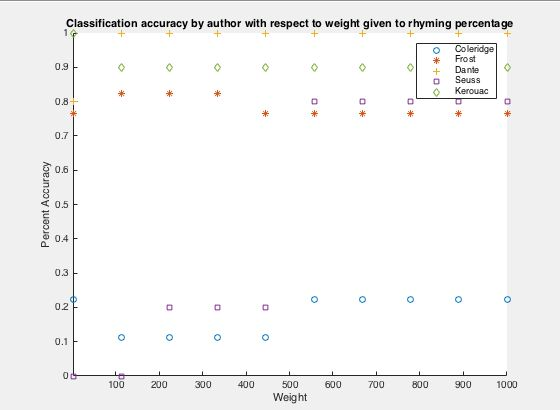
\includegraphics[width=0.8\columnwidth]{class}
\end{figure}

After confirming that our weights make sense, we trained this classifier on half of the poems, and tested it on the other half. We found that our classifier was able to identify the poet of a poem very accurately for certain poets and very poorly for others. The most successful identification was on poems by Dr. Seuss and poems by Jack Kerouac in which we obtained 0\% error in both training and testing data. However, we obtained 100\% error for classifying poems written by the other three poets. After a period of despair, we realized that the number of training examples for Jack Kerouac greatly outnumbered all other poets. The fact that Dr. Seuss poems were able to be correctly separated from Kerouac poems was very impressive given this. The subtleties that made our classifier fail on Coleridge, Dante, and Frost poems would not be remedied without greatly increasing our training set for those poets; however, we decided that focusing on Dr. Seuss and Jack Kerouac poems would have to be an acceptable concession given that classification is an auxiliary goal to generation. 

\subsection{Generation}
Our poem generator was successful in creating poems of appropriate structure, but was not able to consistently produce poems that made syntactic sense. We tested our generator primarily on creating poems in the style of Jack Kerouac’s haikus. The shorter length of these poems made them more practical to produce and analyze in large numbers. 

The weighted random choice of number of lines and number of words in each line was successful in generating poems that were diverse in structure, while still imitating the style of the author’s original work. The generated haikus all had about 2-4 lines and 1-5 words in a line. The domain selection also worked well, so that poems were diverse, but still within the general range of topics about which Kerouac wrote his haikus such as nature, weather, and animals.

Some of the generated poems were very convincing, for example:
\begin{center}
    \textit{
        From thousands of\\
        clouds frost in morning\\
        yellow Moon\\
        in Autumn on the river\\
        }
\end{center}

Compare this with an actual Kerouac haiku (with punctuation removed for comparison):
\begin{center}
    \textit{
        February gales racing\\
        westward through\\
        The clouds the moon\\
        }
\end{center}

The poems have similar imagery, structure, and style. It is not obvious which of the above is the original. Admittedly, it is helpful that Kerouac tended to write in the stream of consciousness style. 

However, many poems were easily recognizable as computer generated. For example:
\begin{center}
    \textit{
        at\\
        the night\\
        in the winter\\
        knocking from the\\
        }
\end{center}

The most glaring issue with this poem is that it ends mid-sentence with a definite article. This reveals a weakness in our program. Because we are only considering bigrams, we have no guarantee that the poem begins or ends with a reasonable word. However, this poem does actually contain reasonable phrases. \textit{"at the night"}, \textit{"in the winter"}, and \textit{"knocking from the"} all are valid, if incomplete, English constructs. 

This, however, exposes another problem with many poems:
\begin{center}
    \textit{
    in the moon in the\\
    blue\\
    and these In the\\
    ditch\\
}
\end{center}

Again, the individual phrases make sense in this poem, but the phrases together do not. Since our factors link only consecutive words, they do not maintain consistency throughout the poem. This highlights that poem generation is not a Markov chain as we have formulated our problem. We could add more information to our state in order to maintain the Markov property, but it would most likely be more appropriate to create factors that scope more than just adjacent variables. 

As a quantitative test, we asked people not invested in this project to attempt to differentiate between our generated Haikus and actual Kerouac Haikus. We attempted to select from a wide variety of individuals to avoid bias. About half of our surveyees were Stanford students whereas the other half were not students. About half worked in the engineering field whereas the other half identified with liberal arts. 

We collected 70 sample points using a set of 10 generated poems, included in the appendix. We chose 10 poems rather than just using one in order to obtain some variety in the generated poems. The generated poems fooled the surveyees 8 times out of these 70 points. Given the grammatical inaccuracies present in the generated poems, these results, while not impressive, were actually better than expected.

\section{Further Work}
\subsection{Morphology}
Our implementation of the generator can be improved by removing the Markov property of our poem generator. As has been shown in our results, poem generation is poorly modeled by a Markov chain. However, we believe that it can still be well modeled by a factor graph. Additional factors such as unary factors at the variables that begin and end a poem would greatly improve the syntactic correctness of our generated poems.

For example, as demonstrated in the results section, many generated poems end or begin inappropriately. This could be solved with the introduction of a unary factor linked to each beginning and terminal word. This factor could bias the assignment towards a specific part of speech or a particular word that has ended or begun one of the poems in the training set.

 Our current implementation should be conducive to adding additional such factors as each factor only needs to output a distribution in the form of a dictionary. There is no inherent difference between a unary factor function and an n-ary factor function in that sense. Other possible factors that could be added include rhyming factors and n-gram factors.
 
\subsection{Generalization}
Currently, our poem generator works best when generating poems in the style of Kerouac. This is mainly due to the fact that Kerouac's haikus are very structured morphologically, and that structure is well characterized by our poem classifier. Additionally, the randomness that characterizes many of Kerouac's haikus currently mesh very well with our bigram factors. However, at the same time, the randomness of Kerouac's haikus also result in very strange generated poems. In order to capture the subtleties of poetry produced by the other poets, we still need to integrate additional features that can capture more arbitrary Language concepts such as sentiment and meter.
\subsection{Integration}
Furthermore, we can improve upon the integration between the poem classifier and the poem generator. For example, as seen in Table \ref{tab:weights}, Dr. Seuss and Robert Frost both have highly positive weights for rhyming percentages when compared to the other poets. So, when generating a Dr. Seuss poem or a Robert Frost poem, we could increase the contribution of a rhyming factor, perhaps by multiplying the distribution returned by some value with magnitude $>1$. Conversely, we could decrease the contribution of the rhyming factor when generating poems from the other poets by multiplying by a reduction constant.

\section{Conclusion}
This project aimed to generate poems in the style of a particular poet by learning the characteristics of the poet from a labeled training set. We have made progress towards this goal and have learned a great deal in the process. We have successfully generated text that is subjectively close to an author's body of work by modeling this problem as a factor graph and utilizing Gibbs sampling. There is definitely a lot more work that can be done, but as a first attempt and as a learning experience, we have reached our goal. 

% references section

% can use a bibliography generated by BibTeX as a .bbl file
% BibTeX documentation can be easily obtained at:
% http://mirror.ctan.org/biblio/bibtex/contrib/doc/
% The IEEEtran BibTeX style support page is at:
% http://www.michaelshell.org/tex/ieeetran/bibtex/
%\bibliographystyle{IEEEtran}
% argument is your BibTeX string definitions and bibliography database(s)
%\bibliography{IEEEabrv,../bib/paper}
%
% <OR> manually copy in the resultant .bbl file
% set second argument of \begin to the number of references
% (used to reserve space for the reference number labels box)
\bibliographystyle{IEEEtran}
\bibliography{final}
\raggedbottom

\pagebreak
\appendix[Survey Poems]
\begin{center}
    \begin{minipage}{\columnwidth}
        \centering
        \begin{tabular}{c|c}
            \textbf{Kerouac} & \textbf{Generated}\\
            \hline
             \begin{minipage}{0.45\columnwidth}  
                 \centering               
                 \textit{
                 america: fishing licenses\\
                 the license\\
                 to meditate\\
                }
                \end{minipage}
             &
             
             \begin{minipage}{0.45\columnwidth}     
                 \centering    
                 \textit{        
                 moon moon thick\\
                 breeze white     \\     
                 snow my chou       \\   
                 chou                 \\ 
                }
                \end{minipage}\\
                
                \hline
                
                
                \begin{minipage}{0.45\columnwidth}  
                    \centering        
                    \textit{       
                    am i a flower	\\
                    bee, that you \\
                    stare at me?    \\ 
                }
                 \end{minipage}
                &
                
                \begin{minipage}{0.45\columnwidth}     
                    \centering            
                    \textit{
                   sit                   \\ 
                   at                     \\
                   storm four bluejays in \\
                   white \\
                }
                \end{minipage}\\
                
                \hline
                
                
                \begin{minipage}{0.45\columnwidth}  
                    \centering        
                    \textit{       
                        a million acres	\\	
                        of bo-trees		\\
                        and not one buddha\\	   
                    }
                \end{minipage}
                &
                
                \begin{minipage}{0.45\columnwidth}     
                    \centering            
                    \textit{
                        of             \\                  
                        the night lay    \\                
                        shore back on boys the night \\                        
                    }
                \end{minipage}\\
                
                \hline
                
                
                \begin{minipage}{0.45\columnwidth}  
                    \centering        
                    \textit{       
                       among the nervous birds\\
                       the morning dove\\
                       nibbles quietly\\                       	   
                    }
                \end{minipage}
                &
                
                \begin{minipage}{0.45\columnwidth}     
                    \centering            
                    \textit{
                       the rainy girl \\
                       of my come     \\
                       birds the moon \\
                       kitty the moon \\                                       
                    }
                \end{minipage}\\
                
                \hline
                
                
                \begin{minipage}{0.45\columnwidth}  
                    \centering        
                    \textit{       
                        a mother \& son\\
                        just took a shortcut\\
                        thru my yard\\                                              	   
                    }
                \end{minipage}
                &
                
                \begin{minipage}{0.45\columnwidth}     
                    \centering            
                    \textit{
                        hope man        \\          
                        a dream of my     \\        
                        slept               \\      
                        wanted should sleeping in \\                                                        
                    }
                \end{minipage}\\
                
                \hline
                
                
                
                
                \begin{minipage}{0.45\columnwidth}  
                    \centering        
                    \textit{       
                       ancient ancient world \\ 
                       - tight skirts      \\
                       by the new car        \\                                                                   	   
                    }
                \end{minipage}
                &
                
                \begin{minipage}{0.45\columnwidth}     
                    \centering            
                    \textit{
                        hens those   \\
                        is           \\
                        made made    \\
                        big and a big\\                                                                               
                    }
                \end{minipage}\\
                
                \hline
                
                
                
                
                \begin{minipage}{0.45\columnwidth}  
                    \centering        
                    \textit{       
                       and the quiet cat\\                       sitting by the post\\
                       perceives the moon\\                                                                                        	   
                    }
                \end{minipage}
                &
                
                \begin{minipage}{0.45\columnwidth}     
                    \centering            
                    \textit{
                        each              \\
                        their out         \\
                        moonlight         \\
                        using for the sky \\                                                                                                      
                    }
                \end{minipage}\\
                
                \hline
                
                
                
                
                \begin{minipage}{0.45\columnwidth}  
                    \centering        
                    \textit{       
                        apassionata sonata\\
                        hiballs, gray\\
                        afternoon in october\\                                                                                        	   
                    }
                \end{minipage}
                &
                
                \begin{minipage}{0.45\columnwidth}     
                    \centering            
                    \textit{
                        the bearded cheek go   \\
                        for the moon in my     \\
                        sighed night           \\
                        log the valley again   \\                                                                                                                      
                    }
                \end{minipage}\\
                
                \hline
                
                
                
                
                \begin{minipage}{0.45\columnwidth}  
                    \centering        
                    \textit{       
                        and as for kennedy 		\\
                        in autumn he slept		\\
                        by swishing peaceful trees\\                                                                                                                	   
                    }
                \end{minipage}
                &
                
                \begin{minipage}{0.45\columnwidth}     
                    \centering            
                    \textit{
                      the boys everyone \\
                      genghiz \\
                      why my boys glancing \\
                      dark in \\                                                                                                                                          
                    }
                \end{minipage}\\
                
                \hline
                
                
                
                
                \begin{minipage}{0.45\columnwidth}  
                    \centering        
                    \textit{       
                        answered a letter\\
                        and took a hot bath\\
                        spring rain\\                                                                                                                                       	   
                    }
                \end{minipage}
                &
                
                \begin{minipage}{0.45\columnwidth}     
                    \centering            
                    \textit{
                        a new fallen on new \\		
                        advanced i            \\       
                        head                    \\     
                        midnight the bushes brooding \\                                                                                                                                                              
                    }
                \end{minipage}\\
                
                \hline
                
             
            
            
        \end{tabular}    
    \end{minipage}
\end{center}



\end{document}


